\documentclass[tikz,border=10pt]{standalone}
\usepackage{tikz}
\usetikzlibrary{shapes.geometric}

\begin{document}
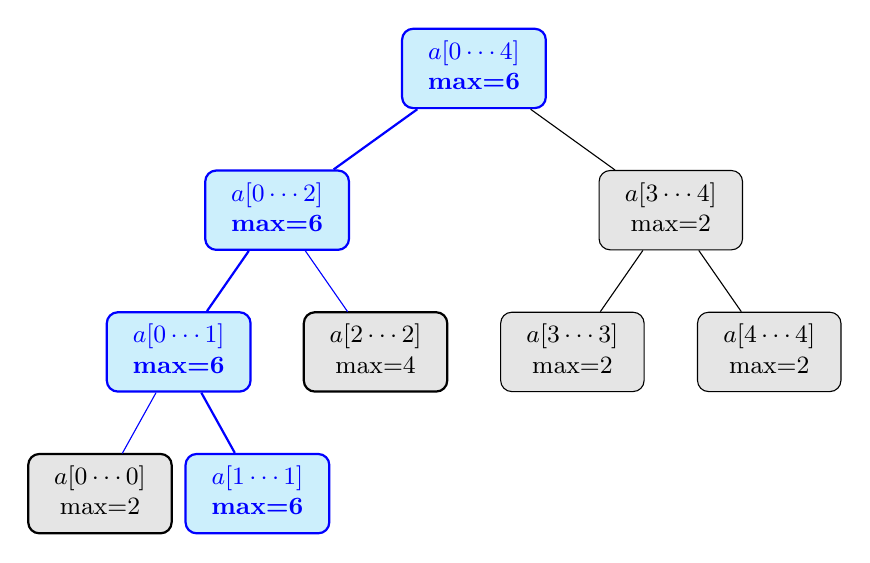
\begin{tikzpicture}[%
  level distance=1.8cm, % Distance between levels
  edge from parent/.style={draw}, % Default edges (overwritten for specific nodes)
  every node/.style={rectangle, rounded corners, draw=black, fill=gray!20, text centered, text=black, font=\small},
  level 1/.style={sibling distance=5cm}, % Wider spacing for first level
  level 2/.style={sibling distance=2.5cm}, % Moderate spacing for second level
  level 3/.style={sibling distance=2cm} % Adjusted spacing for the third level
]

% Root node
\node [draw=blue, fill=cyan!20, text=blue, thick] {%
  \begin{tabular}{c}
    \textbf{$a[0 \cdots 4]$} \\ 
    \textbf{max=6}
  \end{tabular}
}
  % Level 1
  child {node [draw=blue, fill=cyan!20, text=blue, thick] {%
    \begin{tabular}{c}
      \textbf{$a[0 \cdots 2]$} \\ 
      \textbf{max=6}
    \end{tabular}
  }
    % Level 2 (left subtree)
    child {node [draw=blue, fill=cyan!20, text=blue, thick] {%
      \begin{tabular}{c}
        \textbf{$a[0 \cdots 1]$} \\ 
        \textbf{max=6}
      \end{tabular}
    }
      % Level 3 (left subtree of left subtree)
      child {node {%
        \begin{tabular}{c}
          $a[0 \cdots 0]$ \\ 
          max=2
        \end{tabular}
      }
      edge from parent[thin]
      }
      child {node [draw=blue, fill=cyan!20, text=blue, thick] {%
        \begin{tabular}{c}
          \textbf{$a[1 \cdots 1]$} \\ 
          \textbf{max=6}
        \end{tabular}
      }
      edge from parent[thick, draw=blue] % Edge from [0..1] to its children
      }
      edge from parent[thick, draw=blue] % Edge from [0..2] to its children
    }
    child {node {%
      \begin{tabular}{c}
        $a[2 \cdots 2]$ \\ 
        max=4
      \end{tabular}
    }
    edge from parent[thin]
    }
    edge from parent[thick, draw=blue] % Edge from [0..4] to its children
  }
  child {node {%
    \begin{tabular}{c}
      $a[3 \cdots 4]$ \\ 
      max=2
    \end{tabular}
  }
    % Level 2 (right subtree)
    child {node {%
      \begin{tabular}{c}
        $a[3 \cdots 3]$ \\ 
        max=2
      \end{tabular}
    }}
    child {node {%
      \begin{tabular}{c}
        $a[4 \cdots 4]$ \\ 
        max=2
      \end{tabular}
    }}
  };

\end{tikzpicture}
\end{document}